% Q17：按题设得到的分段函数精确绘图，坐标轴及曲线均为矢量。
% 关键点：(-2,0)、(-1,1)、(0,2)、(1,1)、(2,0)。
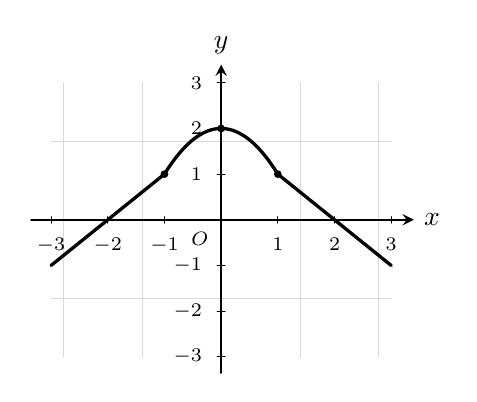
\begin{tikzpicture}[x=0.72cm,y=0.58cm,line cap=round,line join=round,>=stealth]
  % Unit grid matching the original coordinate grid.
  \draw[gray!30,line width=0.25pt] (-3,-3) grid (3,3);
  \draw[->,thick] (-3.35,0)--(3.4,0) node[right] {$x$};
  \draw[->,thick] (0,-3.35)--(0,3.4) node[above] {$y$};

  \foreach \x in {-3,-2,-1,1,2,3}
    \draw (\x,0.07)--(\x,-0.07) node[below=2pt,font=\scriptsize] {$\x$};
  \foreach \y in {-3,-2,-1,1,2,3}
    \draw (0.07,\y)--(-0.07,\y) node[left=2pt,font=\scriptsize] {$\y$};
  \node[below left=1pt,font=\scriptsize] at (0,0) {$O$};

  % f(x)=x+2 for x<=-1, 2-x^2 for -1<x<1, and 2-x for x>=1.
  \draw[very thick] plot[domain=-3:-1,samples=2] (\x,{\x+2});
  \draw[very thick] plot[domain=-1:1,samples=81] (\x,{2-\x*\x});
  \draw[very thick] plot[domain=1:3,samples=2] (\x,{2-\x});
  \foreach \x/\y in {-1/1,0/2,1/1}
    \fill (\x,\y) circle (1.4pt);
\end{tikzpicture}
